\section{Tutorial A4}

\begin{problem}
    Show that if $n, m \in \ZZ^+$, then the equations $z^n = 1 + \i$ and $z^m = 2 - \i$ have no common solutions for $z \in \CC$.
\end{problem}
\begin{solution}
    Seeking a contradiction, suppose there exists some $z \in \CC$ that satisfies the given equations. Then we have \[\abs{z}^n = \abs{1 + \i} = \sqrt{2}\] and \[\abs{z}^m = \abs{2 - \i} = \sqrt{5},\] so \[\abs{z}^{2mn} = 2^m = 5^n,\] but this is a clear contradiction of the Fundamental Theorem of Algebra, so such a $z$ cannot exist, i.e. the two equations have no common solutions.
\end{solution}

\begin{problem}
    Let $z$ and $w$ be complex numbers such that $\abs{z} = \abs{w} = r > 0$. Show that \[\Re{\frac{z+w}{z-w}} = 0.\]
\end{problem}
\begin{solution}
    Let $z = r \e^{\i \t}$ and $w = r \e^{\i \vf}$. Then \[\frac{z + w}{z - w} = \frac{\e^{\i \t} + \e^{\i \vf}}{\e^{\i \t} - \e^{\i \vf}} = \frac{\e^{\i (\t - \vf)/2} + \e^{-\i (\t - \vf)/2}}{\e^{\i (\t - \vf)/2} - \e^{-\i (\t - \vf)/2}} = \frac{2\cos{\frac{\t - \vf}2}}{2\i \sin{\frac{\t - \vf}2}} = -\i \cot{\frac{\t - \vf}{2}},\] which is purely imaginary, so the claim holds.
\end{solution}

\begin{problem}
    Suppose that the complex number $z$ satisfies the equation $5\bp{z + \i}^n = \bp{4 + 3\i} \bp{1 + \i z}^n$. Show that $z$ is purely real.
\end{problem}
\begin{solution}
    Taking the modulus on both sides, we see that \[5 \abs{z + \i}^n = 5 \abs{1 + \i z}^n \implies \abs{z + \i} = \abs{1 + \i z} = \abs{z - \i}.\] The locus of $z$ is the perpendicular bisector of the points representing $\i$ and $-\i$, i.e. the real axis. Hence $z$ is purely real.
\end{solution}

\begin{problem}
    Given that $w + z = w\abs{z}$, where $w, z \in \CC$ with $\abs{w} > 1$, show that \[\bp{\abs{z} + \frac{\abs{w}}{1 - \abs{w}}}\bp{\abs{z} - \frac{\abs{w}}{1 + \abs{w}}} = 0.\]
\end{problem}
\begin{solution}
    Solving for $w$, we get \[w = \frac{z}{\abs{z} - 1} \implies \abs{w} = \frac{\abs{z}}{\abs{\abs{z} - 1}}.\] Note that $\abs{z} \neq 1$, for we would get $w + z = w$, whence $z = 0$, a contradiction. We thus have two cases to examine:

    \case{1}[$\abs{z} - 1 > 0$] Then \[\abs{w} = \frac{\abs{z}}{\abs{z} - 1} \implies \abs{z} = \frac{\abs{w}}{\abs{w} - 1} \implies \abs{z} - \frac{\abs{w}}{\abs{w} - 1} = 0.\]

    \case{2}[$\abs{z} - 1 < 0$] Then \[\abs{w} = \frac{\abs{z}}{1 - \abs{z}} \implies \abs{z} = \frac{\abs{w}}{1 + \abs{w}} \implies \abs{z} - \frac{\abs{w}}{1 + \abs{w}} = 0.\]

    Putting both cases together, we see that \[\bp{\abs{z} + \frac{\abs{w}}{1 - \abs{w}}}\bp{\abs{z} - \frac{\abs{w}}{1 + \abs{w}}} = 0\] as desired.
\end{solution}

\begin{problem}
    Let $z$ be a complex number such that $\abs{z} = 1$. Find the minimum and maximum value of \[\abs{z^5 + \bp{z\conj}^3 + 6z} - 2\abs{z^4 + 1}.\]
\end{problem}
\begin{solution}
    Let $z = \e^{\i \t}$, where $\t \in [0, 2\pi)$. Then
    \begin{align*}
        \abs{z^5 + \bp{z\conj}^3 + 6z} &= \abs{\e^{5 \i \t} + \e^{-3 \i \t} + 6\e^{\i \t}} = \abs{\e^{4\i \t} + \e^{-4\i \t} + 6}\\
        &= \abs{2\cos{4\t} + 6} = \abs{4\cos[2]{2\t} + 4} = 4\cos[2]{2\t} + 4
    \end{align*}
    and \[\abs{z^4 + 1} = \abs{\e^{4\i \t} + 1} = \abs{\e^{2\i\t} + \e^{-2\i\t}} = \abs{2\cos{2\t}}.\] Thus, the given expression is equal to \[\abs{z^5 + \bp{z\conj}^3 + 6z} - 2\abs{z^4 + 1} = 4\cos[2]{2\t} - 4\abs{\cos{2\t}} + 4.\]

    \case{1}[$\cos{2\t} \geq 0$] Then our expression becomes \[4\cos[2]{2\t} - 4\cos{2\t} + 4 = 4\bp{\cos{2\t} - \frac12}^2 + 3,\] which attains a maximum of 4 (when $\cos{2\t} = 1$) and a minimum of 3 (when $\cos{2\t} = 1/2$).

    \case{2}[$\cos{2\t} < 0$] Then our expression becomes \[4\cos[2]{2\t} + 4\cos{2\t} + 4 = 4\bp{\cos{2\t} + \frac12}^2 + 3,\] which once again attains a maximum of 4 (when $\cos{2\t} = -1$) and a minimum of 3 (when $\cos{2\t} = -1/2$).

    Thus, the global maximum is 4, while the global minimum is 3.
\end{solution}

\clearpage
\begin{problem}
    \begin{enumerate}
        \item If $z_1\conj, z_2\conj$ denote the conjugates of the complex numbers $z_1, z_2$, show that $(z_1 + z_2)\conj = z_1\conj + z_2\conj$ and $(z_1z_2)\conj = z_1\conj z_2\conj$.
        \item Given the equation $az + bz\conj = c$, where $a, b , c \in \CC$, deduce the equation $a\conj z\conj + b\conj z = c\conj$. If $\abs{a} \neq \abs{b}$, show that \[z = \frac{a\conj c - b c\conj}{\abs{a}^2 - \abs{b}^2}.\]
        \item If $\abs{a} = \abs{b}$, show that no solution for $z$ exists unless $c = \l\bp{a + b}$ or $c = b \m \i$ for some $\l, \m \in \RR$.
        \item Find the solution for $z$ of the equation \[\bp{7 + \i} z + 5\bp{1 - \i} z\conj = 3 - \i\] in the form $z = p + tq$, where $p$ and $q$ are fixed complex numbers and $t$ is a real parameter.
    \end{enumerate}
\end{problem}
\begin{solution}
    \begin{ppart}
        Let $z_1 = a + b \i$ and $z_2 = c + d\i$, where $a, b, c, d \in \RR$. Then \[\bp{z_1 + z_2}\conj = \bs{\bp{a + c} + \bp{b + d} \i }\conj = \bp{a + c} - \bp{b + d} \i = \bp{a - b \i} + \bp{c - d\i} = z_1\conj + z_2 \conj,\] and \[\bp{z_1 z_2}\conj = \bs{\bp{ac-bd} + \bp{ad + bc}\i}\conj = \bp{ac-bd} - \bp{ad + bc}\i = \bp{a - b\i}\bp{c - d\i} = z_1\conj z_2\conj.\]
    \end{ppart}
    \begin{ppart}
        Taking conjugates, we get \[a\conj z\conj + b\conj z = c\conj.\] We thus get the system of equations \[\left\{\begin{aligned}
            az + bz\conj = c,\\
            a\conj z\conj + b\conj z = c\conj
        \end{aligned}.\right.\] This can be represented with the following matrix equation:\[\begin{pmatrix}[cc]a & b \\ b\conj & a \conj\end{pmatrix}\cvecii{z}{z\conj} = \cvecii{c}{c\conj}.\] Assuming that $\abs{a} \neq \abs{b}$, the determinant of the matrix is \[\det \begin{pmatrix}a & b \\ b\conj & a \conj\end{pmatrix} = aa\conj - bb\conj = \abs{a}^2 - \abs{b}^2 \neq 0,\] so we can invert it to get \[\cvecii{z}{z\conj} = \frac1{\abs{a}^2 - \abs{b}^2} \begin{pmatrix}a\conj & -b \\ -b\conj & a \end{pmatrix} \cvecii{c}{c\conj} \implies z = \frac{a\conj c - b c\conj}{\abs{a}^2 - \abs{b}^2}.\]
    \end{ppart}
    \begin{ppart}
        If $\abs{a} = \abs{b}$, then the determinant of the above matrix is zero, so it is not invertible. We hence turn to Gaussian elimination to solve the matrix equation. Let $a = r\e^{\i \t}$ and $b = r\e^{\i \vf}$. Then \[\begin{pmatrix}[cc|c] a & b & c \\ b\conj & a\conj & c\conj \end{pmatrix} = \begin{pmatrix}[cc|c] r\e^{\i \t} & r\e^{\i \vf} & c \\ r\e^{-\i \vf} & r\e^{-\i \t} & c\conj \end{pmatrix} \rightarrow \begin{matrix}\\ \scriptstyle \e^{\i(\t + \vf)} R_2\end{matrix} \begin{pmatrix}[cc|c] r\e^{\i \t} & r\e^{\i \vf} & c \\ r\e^{\i \t} & r\e^{\i \vf} & c\conj \e^{\i (\t + \vf)} \end{pmatrix}.\] For there to be solutions, we require \[c = c\conj \e^{\i (\t + \vf)} \implies c^2 = \abs{c}^2 \e^{\i (\t + \vf)} = \frac{\abs{c}^2}{r^2} ab \implies c = \l \sqrt{ab}\] for some real $\l$. All that remains is to show that $\sqrt{ab}$ can always be expressed as a real multiple of either $a + b$ or $b\i$.

        Let $\a = \arg{a}$ and $\b = \arg{b}$, with $\abs{a} = \abs{b} = r$.

        \case{1} Suppose $\a \neq \b \pmod{\pi}$. Then \[a + b = r\bp{\e^{\i \a} + \e^{\i \b}} = r\e^{\i (\a + \b)/2} \bs{\e^{\i (\a - \b)/2} + \e^{-\i(\a - \b)/2}} = 2r\cos{\frac{\a - \b}{2}}\e^{\i (\a + \b)/2},\] so \[\arg{a + b} = \frac{\a + \b}{2} = \arg{\sqrt{ab}},\] so $\sqrt{ab}$ is a real multiple of $a + b$ in this case.

        \case{2} Suppose $\a = \b \pmod{\pi}$. Since $\abs{a} = \abs{b}$, we are left with two possibilities: either $a = b$ or $a = -b$. If $a = b$, then we very clearly have \[\frac{\sqrt{ab}}{a + b} = \frac{a}{2a} = \frac12 \in \RR,\] so $\sqrt{ab}$ is a real multiple of $a + b$. Likewise, if $a = -b$, then \[\frac{\sqrt{ab}}{b \i} = \frac{\sqrt{-b^2}}{b \i} = \frac{b\i}{b\i} = 1 \in \RR,\] so $\sqrt{ab}$ is a real multiple of $b\i$.
    \end{ppart}
    \begin{ppart}
        By inspection, \[3-\i = \frac14 \bs{\bp{7 + \i} + \bp{5 - 5\i}},\] so $z = 1/4$ is a particular solution to the above equation. Now consider the associated homogeneous equation: \[\bp{7 + \i} z + \bp{5 - 5\i} z\conj = 0.\] Multiplying by $z$ yields \[z^2 \bp{7 + \i} + \abs{z}^2 \bp{5 - 5\i} = 0 \implies z^2 = \frac{\abs{z^2}}{5} \bp{-3 + 4\i} = \frac{\abs{z}^2}{5} \bp{1 + 2\i}^2.\] Thus, the complementary solution is $z = t \bp{1 + 2\i}$, where $t$ is a real parameter (namely, $t = \abs{z}/\sqrt{5}$). The general solution is thus \[z = \frac14 + t \bp{1 + 2\i}.\]
    \end{ppart}
\end{solution}

\begin{problem}
    The point $P$ represents the complex number $p$ in an Argand diagram, and the points $Q$ and $R$ represent the roots of the equation $(z + p)^2 + n^2 p^2 = 0$, where $n$ is a real positive real constant. Show that
    \begin{enumerate}
        \item $PQ = PR = (4 + n^2)^{1/2} \abs{p}$,
        \item the angle between the lines $PQ$ and $PR$ is $2\arctan{n/2}$.
    \end{enumerate}

    The point $S$ is such that $PQSR$ is a rhombus.
    \begin{enumerate}
        \setcounter{enumi}{2}
        \item Find, in terms of $p$, the complex number represented by $S$.
        \item Find the value of $n$ for which $PQSR$ is a square.
    \end{enumerate}
\end{problem}
\begin{solution}
    \begin{ppart}
        Manipulating the given equation, we see that \[(z + p)^2 + n^2 p^2 = 0 \implies z = - p \pm \i n p.\] Without loss of gerenality, take $q = -p + \i n p$ and $r = -p - \i n p$. Then \[PQ = \abs{q - p} = \abs{-2p + \i np} = \abs{p} \abs{-2 + \i n}.\] and \[PR = \abs{r - p} = \abs{-2p - \i n p} = \abs{p} \abs{2 + \i n}.\] Since $-2 + \i n$ and $2 + \i n$ are reflections of each other in the imaginary axis, their magnitudes are clearly equal, so $PQ = PR$. But \[PR = \abs{p} \abs{2 + \i n} = \abs{p} \sqrt{2^2 + n^2} = \abs{p} \sqrt{4 + n^2},\] so \[PQ = PR = \abs{p} \bp{4 + n^2}^{1/2}.\]
    \end{ppart}
    \begin{ppart}
        Observe that \[\arg{q - p} = \arg{-2p + \i n p} = \arctan{\frac{np}{-2}} = - \arctan{\frac{n}{2}},\] and \[\arg{r - p} = \arg{-2p - \i n p} = \arctan{\frac{-np}{-2p}} = \arctan{\frac{n}{2}}.\] Thus, the difference in the angle between the lines $PQ$ and $PR$ is \[\abs{\arg{q-p} - \arg{r-p}} = \abs{- \arctan{\frac{n}{2}} - \arctan{\frac{n}{2}}} = 2\arctan{\frac{n}{2}}.\]
    \end{ppart}
    \begin{ppart}
        Since $PQSR$ is a rhombus, \[\oa{PS} = \oa{PR} + \oa{RS} = \oa{PR} + \oa{PQ}.\] Rewriting in complex number form, we have \[s - p = \bp{r - p} + \bp{q - p} \implies s = r + q - p = \bp{-p + \i n p} + \bp{-p - \i n p} - p = 3p.\]
    \end{ppart}
    \begin{ppart}
        For $PQSR$ to be a square, the angle between $PQ$ and $PR$ must be $\pi/2$. Thus, \[2\arctan{\frac{n}{2}} = \frac\pi2 \implies n = 2\tan{\frac{\pi}{4}} = 2.\]
    \end{ppart}
\end{solution}

\begin{problem}
    The complex number $z$ has real part $x$ and imaginary part $y$. Show that
    \begin{enumerate}
        \item $\tan{\arg{z-1}} = \frac{y}{x-1}$,
        \item $\tan{\arg{1 - 4/z}} = \frac{4y}{x^2 + y^2 - 4x}$.
    \end{enumerate}

    The points $P$ and $Q$ in an Argand diagram represent $z$ and $4/z$ respectively.
    \begin{enumerate}
        \setcounter{enumi}{2}
        \item Given that the line $PQ$ passes through the point representing $1 + 0\i$, show that \[y = 0 \quad \tor \quad (x-4)^2 + y^2 = 12.\] Sketch the locus of $P$.
        \item Show that, for any position of $P$ on this locus for which $y \neq 0$, \[\abs{1 - \frac1z} = \frac{\sqrt3}{2}.\]
    \end{enumerate}
\end{problem}
\begin{solution}
    \begin{ppart}
        We have \[\tan{\arg{z-1}} = \tan{\arg{(x-1) + \i y}} = \tan \arctan{\frac{y}{x-1}} = \frac{y}{x-1}.\]
    \end{ppart}
    \begin{ppart}
        We have \[\frac{1}{z} = \frac{z\conj}{\abs{z}^2} = \frac{x - \i y}{x^2 + y^2},\] so
        \begin{gather*}
            \tan{\arg{1 - \frac4z}} = \tan{\arg{\frac{x^2 + y^2 - 4x + 4\i y}{x^2 + y^2}}} = \tan \arctan{\frac{4y}{x^2 + y^2 - 4x}}\\
            = \frac{4y}{x^2 + y^2 - 4x}.
        \end{gather*}
    \end{ppart}
    \begin{ppart}
        Note that $P$ and $Q$ are on opposite sides of the real axis (since $\arg{z} = -\arg{4/z}$). Thus, we have \[\arg{1 - \frac4z} = \arg{z-1}.\] From the previous parts, we obtain \[\frac{y}{x - 1} = \frac{4y}{x^2 + y^2 - 4x}.\] Thus, $y = 0$ is clearly a solution. If $y \neq 0$, then further maniupulation yileds \[x^2 + y^2 - 4x = 4x - 4 \implies x^2 - 8x + 16 + y^2 = 12 \implies \bp{x - 4}^2 + y^2 = 12.\]

        \begin{center}\tikzsetnextfilename{464}
            \begin{tikzpicture}[trim axis left, trim axis right]
                \begin{axis}[
                    samples = 101,
                    axis y line=middle,
                    axis x line=middle,
                    xtick = {4},
                    ytick = \empty,
                    xmax=6,
                    xmin=-2,
                    ymin=-5,
                    ymax=5,
                    xlabel = {$\Re$},
                    ylabel = {$\Im$},
                    legend cell align={left},
                    legend pos=outer north east,
                    axis equal,
                    after end axis/.code={
                        \path (axis cs:0,0) 
                            node [anchor=north east] {$O$};
                        }
                    ]

                    \addplot[plotRed, very thick, domain=-20:20] {0};
                    \addlegendentry{Locus of $P$};

                    \draw[plotRed, very thick] (4, 0) circle[radius=2*sqrt(3)];
                    \draw[<->] (4, 0) -- (4, 3.464);
                    \node[anchor=west] at (4, 1.73) {$\sqrt{12}$};
                \end{axis}
            \end{tikzpicture}
        \end{center}
    \end{ppart}
    \begin{ppart}
        Let $R(z)$ be the statement ``the points representing $z$, $4/z$ and 1 are collinear''. Note that this is equivalent to the statement ``the points representing $4/z$, $4/(4/z)$ and 1 are collinear''. Thus, \[R(z) \iff R\of{\frac4z}.\] From the previous part, if $z \in \CC\setminus\RR$, then \[R(z) \implies \abs{z - 4} = \sqrt{12} = 2\sqrt{3}.\] As such, if $R(z)$ is true (i.e. $z$ lies on the locus of $P$), then \[R(z) \implies R\of{\frac4z} \implies \abs{\frac4z - 4} = 2\sqrt{3} \implies \abs{1 - \frac1z} = \frac12 \sqrt3\] as desired.
    \end{ppart}
\end{solution}

\begin{problem}
    The complex numbers $a$, $b$, $c$ are represented in an Argand diagram by the points $A$, $B$ and $C$ respectively. The triangle $ABC$ is equilateral and is labelled anticlockwise. Show that
    \begin{enumerate}
        \item $(c-a) \e^{\i \pi/3} = c - b$,
        \item $(c-a) \e^{-\i \pi/3} = b - a$,
        \item $a^2 + b^2 + c^2 = bc + ca + ab$.
    \end{enumerate}
    
    Given that $a = -4 + 4\i$ and $b = 4-2\i$, use the result in (c) to show that \[(c-\i)^2 = k\bp{3 + 4\i}^2\] where $k$ is real. Hence, find $c$ in exact form.
\end{problem}
\begin{solution}
    \begin{ppart}
        Consider the figure below.

        \begin{center}\tikzsetnextfilename{465}
            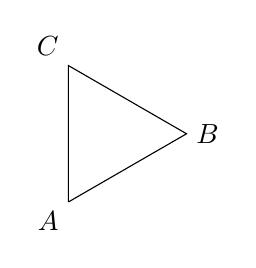
\begin{tikzpicture}
                \coordinate[label=below left:$A$] (A) at (-0.5, -0.866);
                \coordinate[label=right:$B$] (B) at (1, 0);
                \coordinate[label=above left:$C$] (C) at (-0.5, 0.866);

                \draw (A) -- (B) -- (C) -- (A);
            \end{tikzpicture}
        \end{center}

        Clearly, rotating $\oa{AC}$ 60$\deg$ clockwise results in $\oa{BC}$, so \[\bp{c-a} \e^{\i \pi / 3} = c - b.\]
    \end{ppart}
    \begin{ppart}
        Referring to the above figure, we also see that rotating $\oa{AC}$ 60$\deg$ counterclockwise results in $\oa{AB}$, so \[\bp{c - a} \e^{-\i \pi/3} = b - a.\]
    \end{ppart}
    \begin{ppart}
        Multiplying the above two results, we get \[c^2 - 2ac + a^2 = \bp{c-a}^2 = \bp{c-b}\bp{b-a} = cb - ac - b^2 + ab \implies a^2 + b^2 + c^2 = ab + bc + ac.\]
    \end{ppart}

    Using (c), we have \[\bp{-4 + 4\i}^2 + \bp{4 - 2\i}^2 + c^2 = \bp{4 - 2\i}c + \bp{-4 + 4\i} c + \bp{-4 + 4\i}\bp{4 - 2\i},\] which simplifies to \[\bp{c - \i}^2 = c^2 - 2\i c - 1 = -21 + 72\i = 3\bp{-7 + 24\i} = 3\bp{3 + 4\i}.\] Thus, $k = 3$. Taking square roots, we see that $c = \i \pm \sqrt{3} \bp{3 + 4\i}$. Drawing both possibilities on an Argand diagram, along with $a$ and $b$, we reject the negative branch, so $c = \i + \sqrt{3} \bp{3 + 4\i}$.

    \begin{center}\tikzsetnextfilename{466}
        \begin{tikzpicture}[trim axis left, trim axis right]
            \begin{axis}[
                domain = 0:10,
                samples = 101,
                axis y line=middle,
                axis x line=middle,
                xtick = \empty,
                ytick = \empty,
                xmax=8,
                xmin=-8,
                ymin=-8,
                ymax=8,
                axis equal,
                xlabel = {$\Re$},
                ylabel = {$\Im$},
                legend cell align={left},
                legend pos=outer north east,
                after end axis/.code={
                    \path (axis cs:0,0) 
                        node [anchor=north east] {$O$};
                    }
                ]

                \coordinate[label=above left:$A$] (A) at (-4, 4);
                \coordinate[label=below right:$B$] (B) at (4, -2);
                \coordinate[label=below right:$C_+$] (C1) at (5.196, 7.9282);
                \coordinate[label=below left:$C_-$] (C2) at (-5.196, -5.9282);

                \draw (A) -- (B);
                \draw[dashed] (B) -- (C1) -- (A);
                \draw[dashed] (B) -- (C2) -- (A);
            \end{axis}
        \end{tikzpicture}
    \end{center}
\end{solution}

\begin{problem}
    The point $Z$ in an Argand diagram represents the variable complex number $z$, and $a$ is a fixed non-zero complex number.
    \begin{enumerate}
        \item Given that $\abs{z} = \abs{z - 6a}$, sketch the locus of $Z$.
        \item Given that $\abs{z} = 2\abs{z - 3a}$, show that $\abs{z - 4a} = 2\abs{a}$, and hence sketch the locus of $Z$.
    \end{enumerate}

    $P$ and $Q$, represent the complex numbers $p$ and $q$, are the common points of the loci in (a) and (b). Find $\arg{p/q}$, given that it is positive.
\end{problem}
\begin{solution}
    \begin{ppart}
        \begin{center}\tikzsetnextfilename{467}
            \begin{tikzpicture}[trim axis left, trim axis right]
                \begin{axis}[
                    domain = -10:20,
                    samples = 101,
                    axis y line=middle,
                    axis x line=middle,
                    xtick = \empty,
                    ytick = \empty,
                    xmax=15,
                    xmin=-5,
                    ymin=-8,
                    ymax=12,
                    axis equal,
                    xlabel = {$\Re$},
                    ylabel = {$\Im$},
                    legend cell align={left},
                    legend pos=outer north east,
                    after end axis/.code={
                        \path (axis cs:0,0) 
                            node [anchor=north east] {$O$};
                        }
                    ]

                    \coordinate[label=above right:$6a$] (A6) at (12, 6);
                    \coordinate (A3) at (6, 3);
                    \coordinate (O) at (0, 0);

                    \fill (A6) circle[radius=2.5pt];

                    \draw[dashed] (O) --node[sloped]{$|$} (A3);
                    \draw[dashed] (A3) --node[sloped]{$|$} (A6);

                    \addlegendimage{plotRed};
                    \addlegendentry{Locus of $Z$};

                    \addplot[plotRed, very thick] {-2*x + 15};
                \end{axis}
            \end{tikzpicture}
        \end{center}
    \end{ppart}
    \begin{ppart}
        Let $\Lc$ be the locus of $Z$ and $P$ an arbitrary point on $\Lc$. Define $F(3a)$, $A = \Lc \cap OF$, $B = \Lc \cap \bp{OF \text{ extended}}$ and $Q$ on $OP$ extended.

        \begin{center}\tikzsetnextfilename{468}
            \begin{tikzpicture}
                \coordinate[label=below left:$A$] (A) at (2, 0);
                \coordinate[label=below right:$B$] (B) at (6, 0);
                \coordinate[label=below left:$O$] (O) at (0, 0);
                \coordinate[label=above left:$P$] (P) at (4, 2);
                \coordinate[label=above right:$Q$] (Q) at (6, 3);
                \coordinate[label=below:$F$] (F) at (3, 0);

                \draw[plotRed, dotted, thick] (4, 0) circle[radius=2];

                \draw (O) -- (B);
                \draw (O) -- (P);
                \draw[dashed] (P) -- (Q);
                \draw (P) -- (F);
                \draw (P) -- (B);
                \draw (P) -- (A);

                \fill (O) circle[radius=2.5pt];
                \fill (A) circle[radius=2.5pt];
                \fill (B) circle[radius=2.5pt];
                \fill (P) circle[radius=2.5pt];
                \fill (Q) circle[radius=2.5pt];
                \fill (F) circle[radius=2.5pt];

                \node[anchor=north west] at (4.6, -1.8) {$\Lc = \O$};

                \draw pic [draw, angle radius=3mm] {right angle = A--P--B};
            \end{tikzpicture}
        \end{center}

        Since $P, A \in \Lc$, we have \[\frac{OP}{PF} = \frac{OA}{AF} = \frac{\abs{z}}{\abs{z - 3a}} = 2.\] Thus, by the angle bisector theorem, it follows that $\angle APF$ bisects $\angle OPF$.

        Similarly, since $P, B \in \Lc$, we have \[\frac{OP}{PF} = \frac{OB}{BF} = 2.\] Thus, by the angle bisector theorem, it follows that $\angle FPB$ bisects $\angle FPQ$.

        Hence, \[\angle APB = \angle APF + \angle FPB = \frac{\angle OPF + \angle FPQ}{2} = 90\deg.\] Since $P$ is arbitrary, by the converse of Thale's theorem, it follows that $\Lc$ lies on a circle. By symmetry, $OB$ contains the diameter of the circle. Elementary calculations show that $A(2a)$ and $B(6a)$, so the center of the circle is $(2a + 6a)/2 = 4a$ and the radius is $\abs{4a - 2a} = \abs{2a}$. Call this circle $\O$, so $\Lc \subseteq \O$.

        By inverting the above argument and invoking the converse of the angle bisector theorem (and Thale's theorem), we see that $\O \subseteq\Lc$, so we must have $\Lc = \O$. The complex equation for $\O$ (and thus $\Lc$) is given by $\abs{z - 4a} = 2\abs{a}$ as desired.
    \end{ppart}

    \begin{center}\tikzsetnextfilename{469}
        \begin{tikzpicture}[trim axis left, trim axis right]
            \begin{axis}[
                domain = -10:20,
                samples = 101,
                axis y line=middle,
                axis x line=middle,
                xtick = \empty,
                ytick = \empty,
                xmax=13,
                xmin=0,
                ymin=-4,
                ymax=10,
                axis equal,
                xlabel = {$\Re$},
                ylabel = {$\Im$},
                legend cell align={left},
                legend pos=outer north east,
                after end axis/.code={
                    \path (axis cs:0,0) 
                        node [anchor=north east] {$O$};
                    }
                ]

                \coordinate (O) at (0, 0);
                \coordinate[label=below left:$A$] (A) at (4, 2);
                \coordinate[label=right:$B$] (B) at (12, 6);
                \coordinate[label=above right:$F$] (F) at (6, 3);
                \coordinate[label=left:$P$] (P) at (4.26795, 6.4641);
                \coordinate[label=below left:$Q$] (Q) at (7.73205, -0.4641);


                \addplot[plotRed, very thick] {-2*x + 15};
                \draw[plotRed, very thick] (8, 4) circle[radius=4.47];
                \fill (P) circle[radius=2.5pt];
                \fill (Q) circle[radius=2.5pt];

                \fill (A) circle[radius=2.5pt];
                \fill (B) circle[radius=2.5pt];
                \fill (F) circle[radius=2.5pt];

                \draw[dashed] (O) -- (P);
                \draw[dashed] (O) -- (Q);
                \draw[dashed] (O) -- (B);

                \draw pic [draw, angle radius=10mm, "$\t$"] {angle = F--O--P};
                \draw pic [draw, angle radius=12mm, "$\t$"] {angle = Q--O--F};

                \draw pic [draw, angle radius=4mm] {right angle = P--F--O};
                \draw pic [draw, angle radius=3mm] {right angle = Q--F--O};
            \end{axis}
        \end{tikzpicture}
    \end{center}

    Let $\t = \angle POF = \angle QOF$. Then \[\sin \t = \frac{PF}{OF} = \frac{\abs{z - 3a}}{\abs{z}} = \frac12 \implies \t = \frac\pi3.\] Thus, \[\arg{\frac{p}{q}} = \arg{p} - \arg{q} = 2\t = \frac\pi3.\]
\end{solution}

\begin{problem}
    \begin{center}\tikzsetnextfilename{470}
        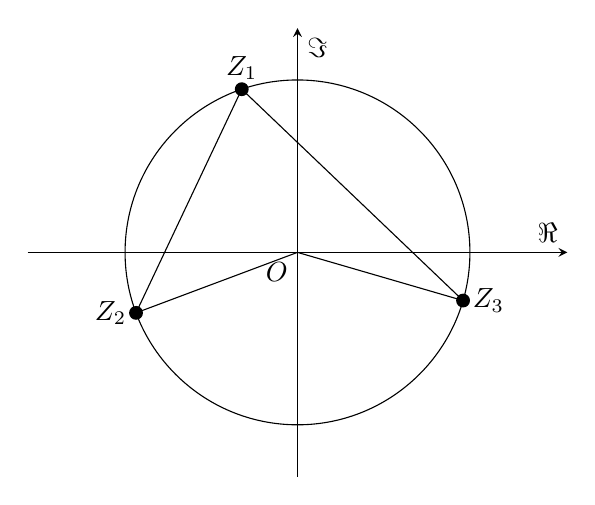
\begin{tikzpicture}[trim axis left, trim axis right]
            \begin{axis}[
                domain = 0:10,
                samples = 101,
                axis y line=middle,
                axis x line=middle,
                xtick = \empty,
                ytick = \empty,
                xmax=1.3,
                xmin=-1.3,
                ymin=-1.3,
                ymax=1.3,
                axis equal,
                xlabel = {$\Re$},
                ylabel = {$\Im$},
                legend cell align={left},
                legend pos=outer north east,
                after end axis/.code={
                    \path (axis cs:0,0) 
                        node [anchor=north east] {$O$};
                    }
                ]

                \coordinate (O) at (0, 0);
                \coordinate[label=above:$Z_1$] (Z1) at (-0.32328957, 0.94630009);
                \coordinate[label=left:$Z_2$] (Z2) at (-0.93645669, -0.35078323);
                \coordinate[label=right:$Z_3$] (Z3) at (0.96017029, -0.2794155);

                \draw (O) circle[radius=1];
                \fill (Z1) circle[radius=2.5pt];
                \fill (Z2) circle[radius=2.5pt];
                \fill (Z3) circle[radius=2.5pt];

                \draw (O) -- (Z3) -- (Z1) -- (Z2) -- (O);
            \end{axis}
        \end{tikzpicture}
    \end{center}

    The complex numbers $z_1 = x_1 + \i y_1$, $z_2 = x_2 + \i y_2$, $z_3 = x_3 + \i y_3$, where $x_k, y_k \in \RR$ and $\abs{z_k} = 1$ for $k = 1, 2, 3$ are represented by the points $Z_1$, $Z_2$ and $Z_3$ on the Argand diagram above.

    \begin{enumerate}
        \item Express the complex numbers $z_1$, $z_2$, $z_3$ in exponential form, where $\a = \arg{z_1}$, $\b = \arg{z_2}$, $\g = \arg{z_3}$.
        \item Using part (a), show that $\arg{z_1 z_2} = \a + \b$.
        \item Without using the property that $\angle Z_2 O Z_3 = 2\angle Z_2 Z_1 Z_3$, find the value of $\angle Z_2 Z_1 Z_3$ in terms of $\b$ and $\g$.
        \item Hence, or otherwise, prove that $\angle Z_2 O Z_3 = 2\angle Z_2 Z_1 Z_3$.
    \end{enumerate}
\end{problem}
\begin{solution}
    \begin{ppart}
        We have \[z_1 = \e^{\i \a}, \quad z_2 = \e^{\i \b}, \quad z_3 = \e^{\i \g}.\]
    \end{ppart}
    \begin{ppart}
        We have \[\arg{z_1 z_2} = \arg{\e^{\i \a} \e^{\i \b}} = \arg{\e^{\i (\a + \b)}} = \a + \b.\]
    \end{ppart}
    \begin{ppart}
        Observe that \[\arg{z_2 - z_1} = \arg{\e^{\i \b} - \e^{\i \a}} = \arg \Big(\e^{\i \frac{\a + \b}{2}} \underbrace{\bp{\e^{\i \frac{\b - \a}{2}} - \e^{-\i \frac{\b - \a}{2}}}}_{2\i \Im \e^{\i \frac{\b - \a}{2}}}\Big) = \frac{\a + \b + \pi}2.\] Similarly, \[\arg{z_3 - z_1} = \arg{\e^{\i \g} - \e^{\i \a}} = \frac{\a + \g + \pi}{2}.\] Thus, \[\angle Z_2 Z_1 Z_3 = \abs{\arg{z_2 - z_1} - \arg{z_3 - z_1}} = \abs{\frac{\a + \b + \pi}2 - \frac{\a + \g + \pi}2} = \abs{\frac{\b - \g}{2}}.\]
    \end{ppart}
    \begin{ppart}
        It is clear that \[\angle Z_2 O Z_3 = \abs{\arg z_2 - \arg z_3} = \abs{\b - \g} = 2\abs{\frac{\b - \g}{2}} = 2\angle Z_2 Z_1 Z_3.\]
    \end{ppart}
\end{solution}

\begin{problem}
    The complex numbers $z_1, z_2, \dots, z_6$ are represented by six distinct points $P_1, P_2, \dots, P_6$ in the Argand diagram. Express the following statements in terms of complex numbers:
    \begin{enumerate}
        \item $\oa{P_1 P_2} = \oa{P_5 P_4}$ and $\oa{P_2 P_3} = \oa{P_6 P_5}$;
        \item $\oa{P_2 P_4}$ is perpendicular to $\oa{P_3 P_6}$.
        \item If (a) holds, show that $\oa{P_3 P_4} = \oa{P_1 P_6}$.
    \end{enumerate}

    Suppose that (a) and (b) both hold, and that $z_1 = 0$, $z_2 = 1$, $z_3 = z$, $z_5 = \i$ and $z_6 = w$.

    \begin{enumerate}
        \setcounter{enumi}{3}
        \item Show that if $P_1 P_2 P_3 P_4 P_5 P_6$ forms a convex hexagon, then $\Re{z} + \Re{w} = 1$ with $\Re{z} > 1$ and $\Re{w} < 0$.
        \item Find the distance between $P_3$ and $P_6$ when $\tan \angle P_3 P_2 P_6 = -2/3$.
    \end{enumerate}
\end{problem}
\begin{solution}
    \begin{ppart}
        We have \[z_2 - z_1 = z_4 - z_5 \quad \tand \quad z_3 - z_2 = z_5 - z_6.\]
    \end{ppart}
    \begin{ppart}
        We have that $z_4 - z_2$ is perpendicular to $z_6 - z_3$. Hence, \[\cvecii{\Re{z_4 - z_2}}{\Re{z_4 - z_2}} \dotp \cvecii{\Re{z_6 - z_3}}{\Im{z_6 - z_3}} = \Re{z_4 - z_2}\Re{z_6 - z_3} + \Im{z_4 - z_2}\Im{z_6 - z_3} = 0.\]
    \end{ppart}
    \begin{ppart}
        Adding both equations in (a), we have $z_3 - z_1 = z_4 - z_6$, so $z_4 - z_3 = z_6 - z_1$, implying $\oa{P_3 P_4} = \oa{P_1 P_6}$.
    \end{ppart}
    \begin{ppart}
        \[w = z_6 = z_5 + z_2 - z_3 = \i + 1 - z \implies w+z = 1 + \i.\] Comparing real parts, we have \[\Re{w} + \Re{w} = 1.\] Now observe that \[z_4 = z_2 - z_1 + z_5 = 1 - 0 + \i = 1 + \i.\] Further, because $\oa{P_2 P_4}$ is perpendicular to $\oa{P_3 P_6}$, we must have $\Im{z} = \Im{w} = 1/2$. We can represent this on the following Argand diagram:

        \begin{center}\tikzsetnextfilename{473}
            \begin{tikzpicture}[trim axis left, trim axis right]
                \begin{axis}[
                    domain = 0:10,
                    samples = 101,
                    axis y line=middle,
                    axis x line=middle,
                    xtick = \empty,
                    ytick = \empty,
                    xmax=1.5,
                    xmin=-0.5,
                    ymin=-0.5,
                    ymax=1.5,
                    xlabel = {$\Re$},
                    ylabel = {$\Im$},
                    legend cell align={left},
                    legend pos=outer north east,
                    ]

                    \coordinate[label=below left:$P_1$] (P1) at (0, 0);
                    \coordinate[label=below:$P_2$] (P2) at (1, 0);
                    \coordinate[label=right:$P_3$] (P3) at (1.3, 0.5);
                    \coordinate[label=above:$P_4$] (P4) at (1, 1);
                    \coordinate[label=above left:$P_5$] (P5) at (0, 1);
                    \coordinate[label=left:$P_6$] (P6) at (-0.3, 0.5);

                    \draw (P1) -- (P2) -- (P3) -- (P4) -- (P5) -- (P6) -- (P1);
                    \draw[dotted] (P3) -- (P6);
                        
                    \fill (P1) circle[radius=2.5pt];
                    \fill (P2) circle[radius=2.5pt];
                    \fill (P3) circle[radius=2.5pt];
                    \fill (P4) circle[radius=2.5pt];
                    \fill (P5) circle[radius=2.5pt];
                    \fill (P6) circle[radius=2.5pt];
                \end{axis}
            \end{tikzpicture}
        \end{center}

        Clearly, for $P_1 P_2 P_3 P_4 P_5 P_6$ to be a convex hexagon, we must have $\Re{w} < \Re{z_1} = 0$ and $\Re{z} > \Re{z_2} = 1$.
    \end{ppart}
    \begin{ppart}
        Since $z_4 - z_3 = z_6 - z_1$, we have $\Re{z_4 - z_3} = \Re{z_6 - z_1}$. Let this modulus of this common value be $a$. Then $z_6 = -a + \i/2$ and $z_3 = 1 + a + \i/2$. It is hence clear that \[\tan \arg z_6 = \frac{1/2}{-a} \quad \tand \quad \tan \arg z_3 = \frac{1/2}{a + 1}.\] Thus, \[-\frac23 = \tan \angle P_3 P_2 P_6 = \tan{\arg z_6 - \arg z_3} = \frac{\tan \arg z_6 - \tan \arg z_3}{1 + \tan \arg z_6 \tan \arg z_3} = \frac{\frac{1/2}{-a} - \frac{1/2}{a + 1}}{1 + \frac{1/2}{-a} \frac{1/2}{a + 1}}.\] Solving, we get \[2a^2 - a - 2 = 0 \implies a = \frac{1 + \sqrt{17}}{4},\] where we reject the negative branch since $a \geq 0$. Thus, \[P_3 P_6 = 2a + 1 = \frac{3 + \sqrt{17}}{2}.\]
    \end{ppart}
\end{solution}

\begin{problem}
    Let $z$, $w$ be complex numbers such that $w = (z-1)/(z+1)$.

    \begin{enumerate}
        \item Prove that $w$ lies within the unit circle in the Argand diagram if and only if $\Re z \geq 0$.
        \item \begin{enumerate}
            \item Suppose that $w$ lies within the unit circle in the Argand diagram. Show that $\abs{1 - w}^2 \Re z = 1- \abs{w}^2$.
            \item Hence, prove that if $\Re z \neq -1$, then $w$ satisfies the equation \[\abs{w - \frac{\Re z}{\Re z + 1}} = \abs{\frac1{\Re z + 1}}.\]
            \item Show instead that if $\Re z = -1$, then $w$ satisfies the equation $w + w\conj -2 = 0$. Hence, explain why the locus representing $w$ is a vertical line passing through $x = 1$.
        \end{enumerate}
    \end{enumerate}
\end{problem}
\begin{solution}
    \begin{ppart}
        For $w$ to lie within the unit circle, we require $\abs{w} \leq 1$, but \[\abs{w} = \frac{\abs{z-1}}{\abs{z+1}} \leq 1 \iff \abs{z-1} \leq \abs{z+1}.\] But this is a standard locus, corresponding precisely to the region of the Argand diagram where the real part is non-negative, so $\abs{w} \leq 1$ if and only if $\Re{z} \geq 0$.
    \end{ppart}
    \begin{ppart}
        \begin{psubpart}
            Note that \[\abs{z+1}^2 = \bp{z+1}\bp{z\conj +1} = \abs{z}^2 + z + z\conj + 1,\] and \[\abs{z-1}^2 = \bp{z-1}\bp{z\conj-1} = \abs{z}^2 - z - z\conj + 1.\] Hence,
            \begin{gather*}
                \frac{1 - \abs{w}^2}{\abs{1 - w}^2} = \frac{1 - \abs{\frac{z-1}{z+1}}^2}{\abs{1 - \frac{z-1}{z+1}}^2} = \frac{\abs{z+1}^2 - \abs{z-1}^2}{\abs{(z+1)-(z-1)}^2} \\
                = \frac{\bp{\abs{z}^2 + z + z\conj + 1} - \bp{\abs{z}^2 - z - z\conj + 1}}{4} = \frac{z + z\conj}{2} = \Re z,
            \end{gather*}
            and we immediately get our desired identity upon clearing denominators.
        \end{psubpart}
        \begin{psubpart}
            From the previous part, we have $\Re{z} \abs{1 - w}^2 = 1 - \abs{w}^2$, so \[\Re{z} \bp{1 - w - w\conj + \abs{w}^2} = 1 - \abs{w}^2.\] Expanding and simplifying, we have \[\bp{1 + \Re{z}} \abs{w}^2 - \Re{z} w - \Re{z} w\conj = 1 - \Re{z}.\] Dividing throughout by $1 + \Re{z}$ yields \[\abs{w}^2 - \frac{\Re{z}}{\Re{z} + 1} w- \frac{\Re{z}}{\Re{z} + 1} w\conj = \frac{1 - \Re{z}}{\Re{z} + 1}.\] Hence, \[\abs{w - \frac{\Re{z}}{\Re{z} +1}}^2 = \frac{1 - \Re{z}}{\Re{z} + 1} + \bp{\frac{\Re{z}}{\Re{z} + 1}}^2 = \frac1{\bp{\Re{z} + 1}^2}.\] The desired result follows immediately.
        \end{psubpart}
        \begin{psubpart}
            If $\Re{z} = -1$, we have \[\abs{w}^2 - 1 = \abs{1 - w}^2 = 1 - w - w\conj + \abs{w} \implies w + w\conj -2 = 0.\] Rewriting, we have \[2\Re{w} = 2 \implies \Re{w} = 1.\] Hence, the locus of $w$ is the vertical line passing through $x = 1$.
        \end{psubpart}
    \end{ppart}
\end{solution}

\begin{problem}
    Let $z_1, z_2$ be complex numbers such that $\arg{z_1}, \arg{z_2} \in (0, \pi/4)$.

    \begin{enumerate}
        \item Show that the function $A(x) = \arctan x$ is an increasing function on $\RR$.
        \item Suppose that $a, b, c, d$ are positive real numbers such that $a/b < c/d$. Prove that \[\frac{a}{b} < \frac{a + c}{b + d} < \frac{c}{d}.\]
        \item Prove that \[\min{\arg{z_1}, \arg{z_2}} < \arg{z_1 + z_2} < \max{\arg{z_1}, \arg{z_2}}.\]
    \end{enumerate}
\end{problem}
\begin{solution}
    \begin{ppart}
        We have \[\der{}{x} A(x) = \frac{1}{1 + x^2} > 0\] for all $x \in \RR$. Hence, $A(x)$ is increasing on $\RR$.
    \end{ppart}
    \begin{ppart}
        Since $a/b < c/d$, we have \[a < \frac{cb}{d} \implies a + c < \frac{cb + cd}{d} \implies \frac{a + c}{b + d} < \frac{c}{d}.\] Similarly, we have \[\frac{ad}{b} < c \implies \frac{ad + ab}{b} < a + c \implies \frac{a}{b} < \frac{a + c}{b + d}.\] Chaining both inequalities yields \[\frac{a}{b} < \frac{a + c}{b + d} < \frac{c}{d}.\]
    \end{ppart}
    \begin{ppart}
        Let $z_1 = b + a\i$, $z_2 = d + c\i$. If $a/b = c/d$, then $z_1$ and $z_2$ are scalar multiples of each other, so \[\arg{z_1 + z_2} = \arg{z_1} \in \bp{0, \frac\pi4}.\] Else, without loss of generality, take $a/b < c/d$. From (b), we know that \[\frac{a}{b} < \frac{a + c}{b + d} < \frac{c}{d}.\] Further, from (a), we can apply $\arctan$ on all sides of the inequality to get \[\arctan \frac{a}{b} < \arctan \frac{a + c}{b + d} < \arctan \frac{c}{d}.\] But \[\arg{z_1} = \arctan \frac{a}{b}, \quad \arg{z_2} = \arctan \frac{c}{d} \quad, \arg{z_1 + z_2} = \arctan \frac{a + c}{b + d},\] so \[\min{\arg{z_1}, \arg{z_2}} = \arg{z_1} < \arg{z_1 + z_2} < \arg{z_2} = \max{\arg{z_1}, \arg{z_2}}.\]
    \end{ppart}
\end{solution}

\begin{problem}
    The complex number $z \neq \i$ satisfies the equation $\abs{z - \i/2} = 1/2$, and $w = \i z / (\i - z)$.
    \begin{enumerate}
        \item Show that $w$ is real.
        \item Show that the points representing $w$, $z$ and $\i$ on the Argand diagram are collinear.
    \end{enumerate}

    Illustrate (a) and (b) on an Argand diagram.
\end{problem}
\begin{solution}
    \begin{ppart}
        Let $z = x + \i y$ where $x, y \in \RR$. The locus of $z$ is a circle centered at $(0, 1/2)$ with radius $1/2$, so \[x^2 + \bp{y - \frac12}^2 = \frac1{2^2} \implies \abs{z}^2 = x^2 + y^2 = y.\] Hence, \[w = \frac{\i z}{\i - z} = \frac{\i z \bp{-\i - z\conj}}{\abs{\i - z}^2} = \frac{z - \abs{z}^2 \i}{\abs{\i - z}^2} = \frac{\bp{x + \i y} - y \i}{\abs{\i - z}^2} = \frac{x}{\abs{\i - z}^2} \in \RR.\]
    \end{ppart}
    \begin{ppart}
        Observe that \[\abs{\i - z}^2 = \bp{\i - z}\bp{-\i - z\conj} = 1 + \abs{z}^2 + \i z - \i z\conj = 1 + y + \i\bp{x + \i y} - \i \bp{x - \i y} = 1 - y.\] Hence, \[\arg{i - w} = -\frac{x}{1 - y} + \i = \arctan \frac{y-1}{x}.\] But \[\arg{\i-z} = \arg{-x + \i(1 - y)} = \arctan \frac{y-1}{x},\] so $\arg{\i - w} = \arg{\i - z}$, from which it follows that the points representing $w$, $z$ and $\i$ on the Argand diagram are collinear.
    \end{ppart}

    \begin{center}\tikzsetnextfilename{472}
        \begin{tikzpicture}[trim axis left, trim axis right]
            \begin{axis}[
                domain = 0:10,
                samples = 101,
                axis y line=middle,
                axis x line=middle,
                xtick = \empty,
                ytick = {0.5, 1},
                yticklabels = {$\frac12 \i$, $\i$},
                xmax=1.25,
                xmin=-0.75,
                ymin=-0.25,
                ymax=1.25,
                axis equal,
                xlabel = {$\Re$},
                ylabel = {$\Im$},
                legend cell align={left},
                legend pos=outer north east,
                after end axis/.code={
                    \path (axis cs:0,0) 
                        node [anchor=north east] {$O$};
                    }
                ]

                \coordinate (I) at (0, 1);
                \coordinate[label=right:$Z$] (Z) at (0.5, 0.5);
                \coordinate[label=below:$W$] (W) at (1, 0);
        
                \draw (W) -- (I);
        
                \draw (0, 0.5) circle[radius=0.5];
                \fill (Z) circle[radius=2.5pt];
                \fill (W) circle[radius=2.5pt];
            \end{axis}
        \end{tikzpicture}
    \end{center}
\end{solution}

\begin{problem}
    Let \[z_k = \cos{\frac{2k\pi}{n}} + \i \sin{\frac{2k\pi}{n}},\] where $k \neq 0$. Show that the set $\bc{(z_k)^t : t = 1, 2, \dots, n}$ has exactly $n$ elements if and only if $k$ and $n$ do not have any common prime factors.
\end{problem}
\begin{solution}
    Let \[\Zc = \bc{(z_k)^t : t = 1, 2, \dots, n} = \bc{\exp{2\pi\i\frac{kt}{n}} : t = 1, 2, \dots, n}.\] Note that the $n = 1$ case is trivial, so we take $n > 1$. It suffices to show that $\abs{\Zc} < n \iff \gcd{n, k} > 1$.

    We begin with the forwards direction. Suppose $\abs{\Zc} < n$. Then there exist distinct $t_1, t_2 \in \bc{1, \dots, n}$ such that $z_k^{t_1} = z_k^{t_2}$. Without loss of generality, suppose $t_1 > t_2$. Then \[\exp{2\pi\i\frac{kt_1}{n}} = \exp{2\pi\i\frac{kt_2}{n} + 2\pi m \i}\] for some integer $m$. Taking logarithms, we have \[2\pi \i \frac{kt_1}{n} = 2\pi \i \frac{kt_2}{n} + 2\pi m \i \implies k\bp{t_1 - t_2} = mn.\] Seeking a contradiction, suppose $\gcd{k, n} = 1$. Then we necessarily have \[n \mid t_1 - t_2.\] But this is impossible, since $1 \leq t_1 - t_2 \leq n-1$. Thus, we conclude that $\gcd{k, n} > 1$ as desired.

    Now, suppose that $\gcd{k, n} > 1$. Define $d = \gcd{n, k}$. Then $n = dn'$ and $k = dk'$ for some integers $n'$ and $k'$. Note that \[d > 1 \implies n' = \frac{n}{d} < n \implies n' + 1 \leq n.\] Additionally, $n' + 1 > 1$. Hence, we can select $t = n' + 1$, whence we get
    \begin{gather*}
        z_k^{n' + 1} = \exp{2\pi \i \frac{k (n' + 1)}{n}} = \exp{2\pi \i \frac{k' (n' + 1)}{n'}} = \exp{2\pi \i k' + 2\pi\i\frac{k'}{n'}}\\
        = \exp{2\pi \i \frac{k'}{n'}} = \exp{2\pi \i \frac{k}{n}} = z_k^{1}.
    \end{gather*}
    But $n' + 1 \neq 1$, so there is a duplicate element in $\Zc$ and we immediately have $\abs{\Zc} < n$.
\end{solution}

\begin{problem}
    \begin{enumerate}
        \item Show that for any $\t \in \RR$, we have \[\sin \t = \frac{2\tan \frac\t2}{1 + \tan^2 \frac\t2} \quad \tand \quad \cos \t = \frac{1 - \tan^2 \frac\t2}{1 + \tan^2 \frac\t2}.\]
        \item Let $z \in \CC$ be a complex number such that $\abs{z} = 1$ and $z \neq -1$. By writing $z$ in trigonometric form, prove that $z = (1+\i t)/(1 - \i t)$ for some $t \in \RR$.
    \end{enumerate}
\end{problem}
\begin{solution}
    \begin{ppart}
        We have \[\frac{2\tan \frac\t2}{1 + \tan^2 \frac\t2} = \frac{2\sin \frac\t2 \cos \frac\t2}{\cos^2 \frac\t2 + \sin^2 \frac\t2} = 2\sin\frac\t2\cos\frac\t2 = \sin \t\] and \[\frac{1 - \tan^2 \frac\t2}{1 + \tan^2 \frac\t2} = \frac{\cos^2 \frac\t2 - \sin^2 \frac\t2}{\cos^2 \frac\t2 + \sin^2 \frac\t2} = \cos^2 \frac\t2 - \sin^2 \frac\t2 = \cos \t.\]
    \end{ppart}
    \begin{ppart}
        We have $z = \cos \t + \i \sin \t$ for some $\t \in [0, 2\pi) \setminus \bc{\pi}$. Let $t = \tan[2]{\t/2}$. Then \[z = \cos \t + \i \sin \t = \frac{1 - t^2 + 2\i t}{1 + t^2} = \frac{\bp{1 + \i t}^2}{\bp{1 + \i t}\bp{1 - \i t}} = \frac{1 + \i t}{1 - \i t}.\]
    \end{ppart}
\end{solution}

\begin{problem}
    Let $z$ be a complex number satisfying the equation $z^n = z + z\conj$ for some positive integer $n$. By expressing $z^n$ in polar form, show that there are exactly $n$ solutions to the equation if and only if $n \not\equiv 1 \pmod{4}$.
\end{problem}
\begin{solution}
    Let $z = r\e^{\i \t}$, where $r \geq 0$ and $\t \in [0, 2\pi)$. Then the given equation can be rewritten as \[r^n \e^{\i n \t} = 2 r \cos \t.\] If $r = 0$, we obtain the trivial solution $z = 0$. For the rest of the proof, we simply take $z \neq 0$, i.e. $r > 0$. Then \[r^{n-1} \e^{\i n \t} = 2 \cos \t,\] which immediately implies $\e^{\i n \t} \in \RR$, so $n \t = k \pi$ for some integer $k$, whence \[r^{n-1} = 2 \bp{-1}^k \cos \frac{k \pi}{n}.\] For $k$ to yield a solution, we require the RHS to be positive, so $k$ must satisfy \[(-1)^k \cos \frac{k \pi}{n} > 0. \tag{$\ast$}\] If $k$ fulfils this condition, then the solution it generates is given by \[z_k = \sqrt[n-1]{2 \bp{-1}^k \cos \frac{k\pi}{n}} \e^{\i k \pi / n}.\] Observe that if $z$ satisfies the given equation, then so must $z\conj$. Hence, the number of solutions given by $\t \in (0, \pi)$ is equal to the number of solutions given by $\t \in (\pi, 2\pi)$. Note also that $\t = \pi/2$ corresponds to the trivial solution $z = 0$. Thus, for the remainder of this proof, we consider only the case where $\t = 0, \pi$ (i.e. $z \in \RR$), $\t \in (0, \pi/2)$ and $\t \in (\pi/2, \pi)$.

    \case{1}[$n \equiv 0 \pmod{4}$] Let $n = 4m$. $\t = 0$ gives the real solution $z = \sqrt[n-1]{2}$, while $\t = \pi$ does not yield any solution (it does not satisfy ($\ast$)). Consider now $\t \in (0, \pi/2)$, i.e. $k = 1, 2, \dots, 2m-1$. For ($\ast$) to hold, we must have $k$ even, so we have $m-1$ valid values of $k$: \[k = 2, 4, \dots, 2m-2.\] Consider now $\t \in (\pi/2, \pi)$, i.e. $k = 2m + 1, 2m+2, \dots, 4m-1$. For ($\ast$) to hold, we must have $k$ odd, so we have another $m$ valid values of $k$: \[k = 2m+1, 2m+3, \dots, 4m-1.\] Now observe that because the first set of $k$'s is even and the second set of $k$'s is odd, the symmetry around $\t = \pi/2$ ($k = 2m$) is broken, so these two sets of $k$'s must yield distinct $z_k$. Altogether, we have a total of $4m = n$ distinct solutions:

    \begin{table}[H]
        \centering
        \begin{tabular}{|c|c|c|}
        \hline
        $\t$ & Unique solutions in interval & Remarks \\ \hline\hline
        0 & 1 & $z = \sqrt[n-1]{2}$ \\ \hline
        $(0, \pi/2)$ & $m-1$ &  \\ \hline
        $\pi/2$ & 1 & $z = 0$ \\ \hline
        $(\pi/2, \pi)$ & $m$ &  \\ \hline
        $\pi$ & 0 &  \\ \hline
        $(\pi, 3\pi/2)$ & $m$ &  Conjugate of $(\pi/2, \pi)$\\ \hline
        $3\pi/2$ & 0 & Counted already ($z = 0$) \\ \hline
        $(3\pi/2, 2\pi)$ & $m-1$ & Conjugate of $(0, \pi/2)$ \\ \hline
        \end{tabular}
    \end{table}

    \case{1}[$n \equiv 2 \pmod{4}$] Let $n = 4m + 2$. $\t = 0$ gives the real solution $z = \sqrt[n-1]{2}$, while $\t = \pi$ does not yield any solution. Consider now $\t \in (0, \pi/2)$, i.e. $k = 1, 2, \dots, 2m$. For ($\ast$) to hold, we must have $k$ even, so we have $m$ valid values of $k$: \[k = 2, 4, \dots, 2m.\] Consider now $\t \in (\pi/2, \pi)$, i.e. $k = 2m+2, 2m+3, \dots, 4m+1$. For ($\ast$) to hold, we must have $k$ odd, so we have another $m$ valid values of $k$: \[k = 2m+3, 2m+5, \dots, 4m+1.\] Once again, the difference in parity between the two sets of $k$'s ensures that they correspond to different $z_k$'s. Altogether, we have a total of $4m+2 = n$ distinct solutions:

    \begin{table}[H]
        \centering
        \begin{tabular}{|c|c|c|}
        \hline
        $\t$ & Unique solutions in interval & Remarks \\ \hline\hline
        0 & 1 & $z = \sqrt[n-1]{2}$ \\ \hline
        $(0, \pi/2)$ & $m$ &  \\ \hline
        $\pi/2$ & 1 & $z = 0$ \\ \hline
        $(\pi/2, \pi)$ & $m$ &  \\ \hline
        $\pi$ & 0 &  \\ \hline
        $(\pi, 3\pi/2)$ & $m$ &  Conjugate of $(\pi/2, \pi)$\\ \hline
        $3\pi/2$ & 0 & Counted already ($z = 0$) \\ \hline
        $(3\pi/2, 2\pi)$ & $m$ & Conjugate of $(0, \pi/2)$ \\ \hline
        \end{tabular}
    \end{table}

    \case{1}[$n \equiv 3 \pmod{4}$] Let $n = 4m + 3$. $\t = 0, \pi$ give the real solutions $z = \pm \sqrt[n-1]{2}$. Consider now $\t \in (0, \pi/2)$, i.e. $k = 1, 2, \dots, 2m+1$. For ($\ast$) to hold, we must have $k$ even, so we have $m$ valid values of $k$: \[k = 2, 4, \dots, 2m.\] Consider now $\t \in (\pi/2, \pi)$, i.e. $k = 2m+2, 2m+3, \dots, 4m+2$. For ($\ast$) to hold, we must have $k$ odd, so we have another $m$ valid values of $k$: \[k = 2m+3, 2m+5, \dots, 4m+1.\] Again, the difference in parity between the two sets of $k$'s ensures that they correspond to different $z_k$'s. Altogether, we have a total of $4m+3 = n$ distinct solutions:

    \begin{table}[H]
        \centering
        \begin{tabular}{|c|c|c|}
        \hline
        $\t$ & Unique solutions in interval & Remarks \\ \hline\hline
        0 & 1 & $z = \sqrt[n-1]{2}$ \\ \hline
        $(0, \pi/2)$ & $m$ &  \\ \hline
        $\pi/2$ & 1 & $z = 0$ \\ \hline
        $(\pi/2, \pi)$ & $m$ &  \\ \hline
        $\pi$ & 1 & $z = -\sqrt[n-1]{2}$ \\ \hline
        $(\pi, 3\pi/2)$ & $m$ &  Conjugate of $(\pi/2, \pi)$\\ \hline
        $3\pi/2$ & 0 & Counted already ($z = 0$) \\ \hline
        $(3\pi/2, 2\pi)$ & $m$ & Conjugate of $(0, \pi/2)$ \\ \hline
        \end{tabular}
    \end{table}

    \case{1}[$n \equiv 1 \pmod{4}$] Let $n = 4m + 1$. $\t = 0, \pi$ give the real solutions $z = \pm \sqrt[n-1]{2}$. Consider now $\t \in (0, \pi/2)$, i.e. $k = 1, 2, \dots, 2m$. For ($\ast$) to hold, we must have $k$ even, so we have $m$ valid values of $k$: \[k = 2, 4, \dots, 2m.\] Consider now $\t \in (\pi/2, \pi)$, i.e. $k = 2m+1, 2m+3, \dots, 4m$. For ($\ast$) to hold, we must have $k$ odd, so we have another $m$ valid values of $k$: \[k = 2m+1, 2m+5, \dots, 4m-1.\] Again, the difference in parity between the two sets of $k$'s ensures that they correspond to different $z_k$'s. Altogether, we have a total of $4m+3 = n+2$ distinct solutions:

    \begin{table}[H]
        \centering
        \begin{tabular}{|c|c|c|}
        \hline
        $\t$ & Unique solutions in interval & Remarks \\ \hline\hline
        0 & 1 & $z = \sqrt[n-1]{2}$ \\ \hline
        $(0, \pi/2)$ & $m$ &  \\ \hline
        $\pi/2$ & 1 & $z = 0$ \\ \hline
        $(\pi/2, \pi)$ & $m$ &  \\ \hline
        $\pi$ & 1 & $z = -\sqrt[n-1]{2}$ \\ \hline
        $(\pi, 3\pi/2)$ & $m$ &  Conjugate of $(\pi/2, \pi)$\\ \hline
        $3\pi/2$ & 0 & Counted already ($z = 0$) \\ \hline
        $(3\pi/2, 2\pi)$ & $m$ & Conjugate of $(0, \pi/2)$ \\ \hline
        \end{tabular}
    \end{table}
\end{solution}

\begin{problem}
    Let \[w = \frac{z-s}{1 - s\conj z},\] where $z = \e^{2\pi \i / 3}$ and $s$ is a complex number such that $\pi/2 < \arg s < 2\pi/3$ and $\abs{s} = \abs{z - s}$. Show that $\abs{w} = 1$ and $2\pi/3 < \arg{w} < \pi$.
\end{problem}
\begin{solution}
    We note that $z\conj = 1/z$, so \[w = \frac{z-s}{1 - s\conj z} = \frac{z-s}{z\bp{1/z - s\conj}} = \frac{z-s}{z \bp{z\conj - s\conj}} = \frac{z-s}{z\bp{z - s}\conj}.\] From here, we easily conclude that \[\abs{w} = \frac{\abs{z-s}}{\abs{z} \abs{(z-s)\conj}} = \frac{\abs{z-s}}{\abs{(z-s)\conj}} = 1.\]

    Next, we observe that \[\arg w = \arg{z-s} - \arg{z} - \arg{(z-s)\conj} = 2\arg{z-s} - \frac{2\pi}3.\] Consider now the locus of $s$. Let $W(w)$, $A(w/2)$ and $B(\i/\sqrt3)$. One can verify that $w/2$ and $\i/\sqrt3$ are the solutions to $\arg{s} = \arg{z-s}$ when $\arg s = 2\pi/3, \pi/2$ respectively.

    \begin{center}\tikzsetnextfilename{471}
        \begin{tikzpicture}[trim axis left, trim axis right]
            \begin{axis}[
                domain = 0:10,
                samples = 101,
                axis y line=middle,
                axis x line=middle,
                xtick = \empty,
                ytick = \empty,
                xmax=0.25,
                xmin=-0.75,
                ymin=-0.25,
                ymax=1,
                axis equal,
                xlabel = {$\Re$},
                ylabel = {$\Im$},
                legend cell align={left},
                legend pos=outer north east,
                after end axis/.code={
                    \path (axis cs:0,0) 
                        node [anchor=north east] {$O$};
                    }
                ]

                \coordinate[label=above left:$W$] (W) at (-0.5, 0.866);
                \coordinate[label=left:$A$] (A) at (-0.25, 0.433);
                \coordinate[label=below right:$B$] (B) at (0, 0.577);
                \coordinate (O) at (0, 0);
                \coordinate (Z) at (0.5, 0.577);
                \coordinate (Y) at (0.5, 0.433);
        
                \draw[dashed] (O) -- (W) -- (B);
                \draw[plotRed, very thick] (A) -- (B);
                \draw[dotted] (Z) -- (B);
                \draw[dotted] (Y) -- (A);

                \addlegendimage{plotRed, very thick};
                \addlegendentry{Locus of $s$};

                \draw[dashed] (O) --node[sloped]{$|$} (A);
                \draw[dashed] (A) --node[sloped]{$|$} (W);
                \draw[dashed] (O) --node[sloped]{$||$} (B);
                \draw[dashed] (B) --node[sloped]{$||$} (W);
        
                \fill (W) circle[radius=2.5pt];
                \draw[plotRed] (A) circle[radius=2.5pt];
                \draw[plotRed] (B) circle[radius=2.5pt];

                \draw pic [draw, angle radius=4mm] {angle = Y--A--W};
                \draw pic [draw, angle radius=4mm] {angle = Z--B--W};
            \end{axis}
        \end{tikzpicture}
    \end{center}

    From the above diagram, it is clear that $\inf \arg{z-s}$ is attained at $A$, so \[\inf \arg{z-s} = \frac{2\pi}3.\] Meanwhile, $\sup \arg{z-s}$ is attained at $B$. Using the property that $\abs{s} = \abs{z-s}$, we see that $\triangle OBW$ is isosceles, with \[\angle BOW = \angle BWO = \arg w - \frac\pi2 = \frac\pi6.\] Hence, $\angle WBO = \pi - 2(\pi/6) = 2\pi/3$, whence \[\sup \arg{z-s} = 2\pi - \frac{2\pi}3 - \frac\pi2 = \frac{5\pi}6.\]

    Thus, \[\arg{z-s} \in \bp{\frac{2\pi}3, \frac{5\pi}6} \implies \arg w = 2\arg{z-s} - \frac{2\pi}3 \in \bp{\frac{2\pi}3, \pi}.\]
\end{solution}